\documentclass[11pt]{article}
\usepackage[margin=1in]{geometry}
\usepackage[utf8]{inputenc}
\usepackage[T1]{fontenc}
\usepackage{amsmath,amssymb}
\usepackage{booktabs}
\usepackage{graphicx}
\usepackage{xcolor}
\usepackage[numbers,sort&compress]{natbib}
\usepackage{hyperref}
\usepackage{caption}
\setlength{\parskip}{0.4em}
% Citations are placeholders until verified: \unv{} prints a visible flag (see docs/paper/OUTLINE.md, section 5).
\newcommand{\unv}[1]{\textcolor{red}{[UNVERIFIED: #1]}}
\newcommand{\todo}[1]{\textcolor{blue}{[TODO: #1]}}
\newcommand{\laya}{\textsc{Laya}}

\title{When does a frozen pretrained decision model help evolved agents?\\
\large Pre-registered evidence from a consequence-delay ecology}
\author{Feng Yu\\Independent researcher}
\date{Draft \today}

\begin{document}
\maketitle

\begin{abstract}
A frozen pretrained model can supply a prior judgement about what to eat before an agent has eaten anything, but it is unclear how much evolved agents should trust it, and when it helps. We build a controlled ecology in which innate parameters, lifetime learning and a frozen model's judgements can be separated, with delayed and deceptive consequences, language cues that change over time, and social observation. Using pre-registered, hash-frozen evaluations of 228 independently evolved genomes, we find that the net value of the prior is conditional: it is neutral without a delay in consequences, grows with the delay (about $+0.04$ to $+0.05$ in fitness at 40 ticks and $+0.07$ at 80 ticks, in every seed), and is absent when experience alone can solve the task. The frozen model beats a sentiment lexicon only where descriptions require world knowledge, and the trust learned for it transfers across dialects while that learned for the lexicon does not. Individuals with a prior use language cues from neighbours and ripening stages and lose when the cues are wrong. We also report null and negative results, including an early large effect that did not replicate across training seeds. The setting is a simulation with templated scenarios written by one author, and the evidence is limited by small numbers of seeds.
\end{abstract}

\section{Introduction}
\todo{Write after Methods and Results. Plan: docs/paper/PLAN.md, section Introduction (P1--P6). Cite only verified references.}

\section{Related work}
\label{sec:related}

\paragraph{Evolution and learning.}
That learning can guide evolution without any inheritance of acquired traits was shown in simulation by \citet{hinton1987}; \citet{fontanari2017} argue that those simulations demonstrated the selection of learning ability rather than the Baldwin effect proper, and estimate the probability and time with which a learned behaviour becomes innate. \citet{ackley1992} combined evolution and learning in an artificial environment of adaptive and non-adaptive organisms and report that the combination was more successful than either alone; \citet{le2019baldwin} report a similar result for self-taught neural networks in a multi-agent foraging and survival simulation. \citet{roupassov2026} provide an open-source reimplementation of a 1992 artificial-life testbed for evolutionary reinforcement learning and compare neural with programmatic policies using survival analysis over 4,000 trials. Our individuals resemble programmatic policies (a fixed rule skeleton with a few evolved parameters), and our setting adds a third source of competence that none of these studies includes: a frozen pretrained model whose judgements are fixed and whose contribution can be switched off, shuffled or replaced.

\paragraph{Language models as priors for agents.}
\citet{yan2025llmprior} treat a language model as a prior over actions and integrate it into reinforcement learning through Bayesian inference, reporting a large reduction in required samples in offline settings. \citet{arumugam2025} have language models implement posterior sampling to improve exploration. \citet{murugesan2020} use commonsense knowledge from ConceptNet to let agents in text-based games filter implausible actions. These studies ask whether a prior speeds up learning; they do not separate the contribution of an evolved genome from that of learning, and they do not test the conditions under which a prior is neutral or unnecessary. A different line uses language models inside evolutionary search: \citet{lehman2022} use a code model as a mutation operator, and \citet{sygkounas2026} co-evolve language-model-generated policies and environments. In our work the model is not part of the search; it supplies fixed judgements that evolved genomes learn how much to trust. The frozen model we use, \laya{}, is described by its model card as a base to be specialised rather than a zero-shot decision engine \citep{laya}; we report, under our setting and with a correction for its preference for the first option, how well its zero-shot judgements of food descriptions separate nutritious from toxic ones (Section~\ref{sec:res-quality}). Its encoder is ModernBERT \citep{warner2024}.

\paragraph{Delayed consequences.}
In animals, an aversion to a food can be learned even when illness follows long after eating, and the cue that becomes associated depends on the kind of consequence \citep{garcia1966}; \citet{kalat1973} proposed that the long delay is bridged by ``learned safety'': during the delay the animal learns that the familiar taste is safe. Our credit-window gene, which attributes a delayed shock to foods eaten shortly before, is an engineering analogue of the problem these studies describe; we make no claim that our individuals model the biological mechanism.

\paragraph{Evaluation practice.}
Pre-registration separates predictions from post hoc analyses \citep{nosek2018}. In reinforcement learning the number of random seeds determines the risk of statistical errors \citep{colas2018}; we treat the training seed as the unit of analysis, state effect-size thresholds in advance, and use evolution strategies \citep{salimans2017} for training. As a sentiment baseline we use the VADER lexicon \citep{hutto2014}.

\section{The ecology, the frozen model, and the individuals}
\label{sec:methods}

We study whether a frozen pretrained decision model, used as a source of prior judgements about food descriptions, helps individuals whose decision-layer parameters are evolved and whose beliefs are learned within a lifetime. The design goal is that three sources of competence can be separated: \emph{innate} parameters (the genome of an individual), \emph{acquired} knowledge (beliefs formed from the individual's own experience), and \emph{perception} supplied by a frozen model whose weights are never changed. Evolution of the genome is not evolution of the frozen model.

\subsection{The ecology}
\label{sec:ecology}
A shared simulator owns the world state. Individuals (the cohort) only submit action proposals; energy, position and survival are changed exclusively by the simulator, and an energy ledger (initial energy plus supply equals living energy, stored food, and every recorded loss) is verified after each step in the test suite. World time does not depend on rendering. Randomness comes from simulator-managed generators, and a run is reproducible from its configuration and the recorded actions.

Unless stated otherwise, the world is a $16\times 12$ grid with eight individuals and a horizon of 3600 ticks, with one decision every ten ticks (360 rounds). An individual has capacity 40, starts with 32 units of energy and pays a resting metabolism of 0.012 per tick and a movement cost per unit distance. Food (140 units initially, 14 units added every ten ticks to random cells) decays at 0.003 per tick; there is no diffusion, no reproduction and no return of energy at death, so the cohort is fixed and the energy budget is closed. An individual sees only the cells within a perception radius of three, a memory of recently seen food (at most eight entries), and its own state; it never sees global positions or hidden properties of other individuals. A small discrete action set (move, eat, rest) is available. Eating transfers at most 0.6 units per tick from the current cell.

\paragraph{Semantic food.}
Each food-bearing cell carries one \emph{kind}. The kind has a natural-language description that is visible to individuals and a hidden effect factor $f$: eating an amount $a$ changes the individual's energy by $af$. Factors are drawn from four tiers: nutritive ($f=+1$), mild ($-0.4$), strong ($-1$) and lethal ($-4$); in all experiments reported here the lethal tier is allowed (damage cap 4). A world samples $K$ kinds (32 by default), half nutritive and half toxic, where, among toxic kinds, 15\% are lethal, 40\% strong and 45\% mild. \emph{Deception} flips the true effect of a fraction of kinds ($25\%$ or $40\%$) without changing their description: a nutritive description may hide a harmful effect, and a toxic description a nutritive one. Hidden factors are used only by the simulator to settle energy and by the oracle (Section~\ref{sec:individuals}) to measure ceilings; they never enter any individual's input, feature or training signal.

\paragraph{Descriptions and dialects.}
Descriptions are produced by a generator that is independent of any model output. Each kind has a hidden tier, and its text is composed of two or three clauses drawn from five fields (appearance, smell, feel, place, signs). A clause is a positive, negative, or neutral phrase; with probability 0.9 it agrees with the truth, and 20\% of clauses are replaced by an uninformative phrase. We wrote four dialects with disjoint phrasing: a \emph{training} dialect (12,000 descriptions), a \emph{test} dialect (4,000), a \emph{held-out} field-notes dialect (4,000, written blind to any model output) and a \emph{factual} dialect (4,000, neutral in tone, whose clues are facts and indirect knowledge such as related species, habitat, animal behaviour and the effect of cooking). For the factual dialect we also generated a separate 12,000-description training pool that shares the clause bank with, but contains no text identical to, the evaluation pool. All dialects were written by one author; this is a limitation (Section~\ref{sec:limitations}).

\paragraph{Delayed consequences.}
With a delay of $d$ ticks, the energy effect of a bite lands only after $d$ ticks. Until then the gain is recorded as \emph{in transit} in the ledger (and is lost if the individual dies first), and when the effect lands the individual perceives a one-sentence sensation (for example, ``a dull ache stirs in your belly''). We use $d\in\{0,20,40,80\}$.

\paragraph{Ripening and seasons (language cues that change over time).}
In the ripening world the effect of a nutritive kind depends on a stage that cycles with time: the season is $\lfloor t/300\rfloor \bmod 4$ and each kind has a fixed phase offset. The four stages multiply the factor of nutritive kinds by $0.3$ (unripe), $1$ (ripe), $0.4$ (overripe) and $-0.8$ (rotten); toxic kinds do not change. The description shown to the individual is the base description followed by a stage phrase (for example, ``gone soft and sour''), and the observation carries a season sentence that never states a value. Two phrasings of the four stage phrases exist: set A is used for training and set B for evaluation. A cue can be \emph{true}, \emph{absent} (the value still follows the stage) or \emph{mismatched} (the phrase of stage $s+2$ is shown), which changes observations but never the settlement. We use $K=16$ (a hard world) and $K=4$ (a world that experience-only learners can solve; Section~\ref{sec:results}).

\paragraph{Social observation.}
When enabled, a visible neighbour is accompanied by a one-sentence description of its appearance (for example, ``doubled over, clutching its belly''), chosen from a bank according to its most recent noticeable consequence (at least 0.3 energy, about half a bite; when delayed, at the time the effect lands), and by the descriptions of up to three foods it ate in the last 300 ticks. Appearances persist for 60 ticks. Individuals do not share parameters, beliefs or internal experience. Appearance phrases also come in two sets (A for training, B for evaluation) and can be true, absent or mismatched (benefit and harm swapped).

\subsection{The frozen model as ``System 1''}
\label{sec:laya}
The frozen model is \laya{} (a ModernBERT-large encoder with a fine-tuned two-layer decision head, about 421M parameters) \unv{Laya model card and the Jev/Laya documentation}. It is used only as a source of cached judgements and representations: for each food description we ask whether the creature should eat the food, in two option orders, and average the probability of ``eat'' (the head has a strong preference for the first option, which the two-order average removes). The result, a probability $p$ per description text, is cached and read by individuals as a prior; the model is not called in the simulation loop. We also cache the encoder's mean-pooled representation of each description, projected to 32 dimensions with a PCA fitted on the training dialect only, for the experiments that use embeddings. All cached values depend on the text alone.

\subsection{Individuals and genomes}
\label{sec:individuals}
Individuals are \emph{structured}: a fixed rule skeleton moves toward allowed food and eats (a rule that was validated before any evolution), and the genome controls how the individual treats priors and experience. An individual keeps a belief for each description it has eaten, $(n,s)$ (the number of experiences and their sum), updated with the realised energy gain $x=\mathrm{clip}(\mathrm{gain}/3,-1,1)$ and with a forgetting rate. The value of a description $d$ is
\begin{equation}
v(d)=\frac{n_0\,v_0(d)+s}{n_0+n}+\frac{c}{1+n},\qquad v_0(d)=\mathrm{clip}\bigl(a\,(2p_d-1)+b_0\bigr),
\end{equation}
where $n_0=e^{g_1}$ is the trust in the prior (a pseudo-count), $c$ a curiosity bonus, and $a,b_0$ a calibration slope and bias applied to the prior $p_d$. Foods with $v<\tau$ are vetoed (hidden from the skeleton), except for a retry probability. Further genes set the forgetting rate, the minimum energy fraction required before trying an unseen food, and, in delayed worlds, a \emph{credit window}: when a large energy shock arrives, the individual credits it to every kind eaten in the preceding window (up to 150 ticks). The base genome has nine genes; social individuals have one more (the weight of social evidence, Section~\ref{sec:ecology}).

\paragraph{Prior conditions.}
The \emph{prior source} defines $p_d$: \texttt{laya} (the cached judgement above), \texttt{none} ($v_0=0$, so the individual learns from experience only), \texttt{vader} (the valence lexicon VADER \unv{Hutto and Gilbert, VADER}, squashed to $[0,1]$, as an independent sentiment baseline), and \texttt{shuffled} (the cached judgements assigned to other descriptions, which preserves their distribution but destroys the correspondence). A hand-written oracle that reads the hidden factors, and a blind rule that eats everything it reaches, are used only to bound the achievable range; the oracle never produces an individual.

\paragraph{Social individuals.}
A social individual wraps each neighbour appearance as a sentence about a food (``a food that a nearby creature just ate; the creature now looks \dots'') and reads it with the same prior source as the food descriptions. When the reading is clearly favourable or unfavourable, the neighbour's recent meals receive one weighted piece of evidence (the weight is the social gene); the same appearance and meals count once within 120 ticks, because neighbours have no identity across decisions. An individual with no prior cannot read the sentence and ignores neighbours.

\subsection{Evolution}
\label{sec:evolution}
Genomes are optimised with an evolution strategy \unv{Salimans et al., OpenAI-ES}: antithetic sampling, rank-based fitness shaping, an Adam update, normalised gene coordinates, population 24, perturbation scale 0.25 and learning rate 0.1, for 40 generations. Each generation evaluates every candidate on six training worlds drawn from the training dialect (the deception rate alternates between 0.25 and 0.40 where stated), and the cohort of eight identical individuals shares the genome. Fitness is $0.7\times$(fraction of agent-ticks survived)$+0.3\times$(final energy as a fraction of capacity), averaged over the cohort. The training world sequence is the same for every evolutionary run; runs differ in the noise of the strategy, and the ``training seed'' pairs the same noise across conditions. \emph{Matched} training means that training and evaluation share the consequence delay (and, where relevant, the cue structure).

\section{Evaluation protocol}
\label{sec:protocol}

\subsection{Pre-registration workflow}
Every confirmatory comparison reported in this paper follows the same sequence. (1)~A protocol is written and committed to the repository before the individuals under test are trained: the systems, the training command, the evaluation worlds (including their random seeds), the hypotheses with effect-size thresholds, the statistics and the known limitations. (2)~The individuals are trained and none is selected, excluded or retrained. (3)~The SHA-256 hashes of all evolved genomes are written and committed. (4)~The evaluation script, which refuses to run if any hash differs from the committed one, is run \emph{once}. (5)~Results are recorded as they are, including those that contradict the hypotheses. Git commits supply the time stamps. Pre-registrations are numbered 02--11 in the repository, in the order in which they were written. Development-phase experiments, which informed the design of later protocols, are labelled as such and are not used as confirmatory evidence.

Two procedural deviations are disclosed. In pre-registration 04 the stepwise rule did not anticipate tied $p$ values (Section~\ref{sec:results}), and from pre-registration 06 the Holm step-down uses $p$ values only, with the effect-size condition applied to each hypothesis separately. In pre-registration 09 the hash commit was made after, not at, the end of training (the code and the genomes are unchanged, verified by the hashes of the source files recorded in each training manifest), and evaluation was split into eight shards run in parallel, checked against a single-process run on 36 worlds.

\subsection{Unit of analysis and statistics}
The unit of analysis is the \emph{training seed}: the same evolutionary noise sequence is used for every condition, so a comparison is a paired difference between conditions that share a seed. For each seed we average fitness over the evaluation worlds (two deception levels with 32 worlds each, over one or two evaluation pools) and take the difference between the two conditions. With $n$ seeds, the test of a positive mean difference is the exact one-sided sign-flip test: the $p$ value is the fraction of the $2^n$ sign assignments whose mean is at least the observed mean, so with $n=8$ the smallest attainable value is $1/256\approx 0.0039$. Where the claim is non-inferiority, the differences are shifted by the margin first. Hypotheses within a pre-registration are corrected with the Holm step-down at a total level of 0.05. A hypothesis is \emph{supported} only if it is rejected by the Holm procedure \emph{and} its mean difference meets its own pre-registered threshold. Confidence statements about magnitude use percentile bootstrap intervals over the training seeds (20,000 resamples); with three to eight seeds these intervals are rough, and we report them only as descriptions.

Pre-registrations 02 and 03 predate this design: they resample worlds within seeds (02) or require significance in each of three training seeds (03). We keep their formal outcomes and report them as stated.

\subsection{Tiered reading of results}
A single pass/fail verdict conflates direction and size. We therefore also report, after the fact, a tiered reading of each comparison (Appendix, Table~\ref{tab:tiers}): \emph{direction confirmed} when all seeds have the same sign; \emph{magnitude confirmed} when the lower bound of the seed-level interval reaches the pre-registered threshold, \emph{magnitude unclear} when the interval contains it, and \emph{magnitude below threshold} when the upper bound lies below it; \emph{non-inferiority confirmed} when the lower bound exceeds the margin. This reading does not change any formal outcome. Its purpose is to prevent two errors: reading ``not supported'' as ``no effect'' when a small effect is certain in sign, and reading ``supported'' as ``large'' when the interval is wide.

\subsection{Evaluation pools and reuse}
Evaluation uses held-out dialect pools whose descriptions never appear in training. The held-out field-notes pool was evaluated in several pre-registrations (only summary statistics were inspected; it was never used to tune a design or to select a genome), so it is no longer an untouched sample. Where a new comparison needs an untouched pool, we use the factual-dialect pool, which was first used for a prior-quality evaluation and then for individuals in pre-registration 06. Hypothesis tests are not corrected across pre-registrations; in total 228 independent evolutionary runs contribute to the confirmatory comparisons (12 in pre-registrations 02--03, 24 in 04, 48 in each of 06 and 07, and 24 in each of 08--11).

\section{Results}
\label{sec:results}

All numbers are differences in fitness (Section~\ref{sec:evolution}), averaged over evaluation worlds within each training seed; intervals are percentile bootstrap intervals over training seeds (Section~\ref{sec:protocol}). Figure~\ref{fig:forest} summarises the main confirmatory comparisons and Table~\ref{tab:confirmatory} lists every hypothesis with its formal outcome; Appendix Table~\ref{tab:tiers} gives the tiered reading. We describe the results in the order of the questions they answer; a result is called \emph{conditional} when it holds only under a stated delay, dialect or cue structure.

\begin{figure}[t]
\centering
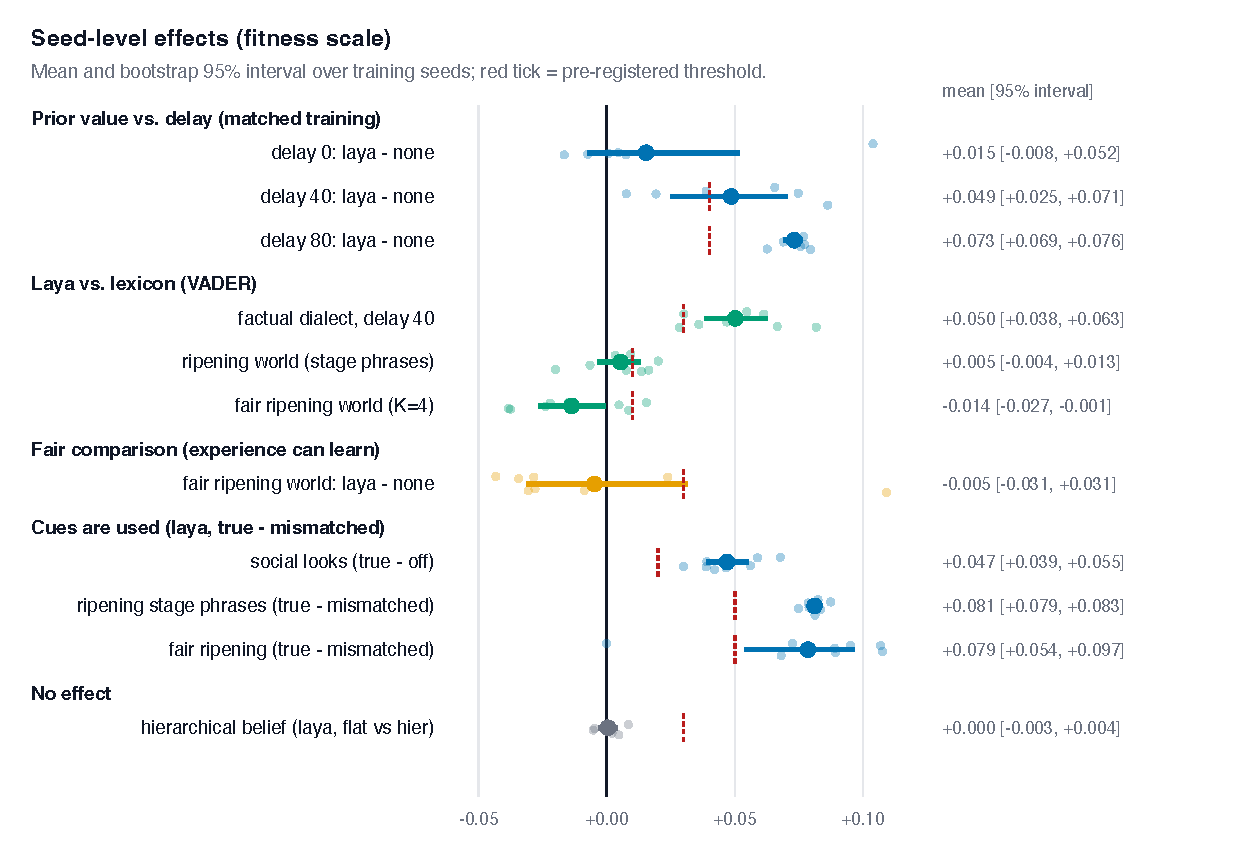
\includegraphics[width=\textwidth]{figures/fig1_forest.pdf}
\caption{Seed-level effects of the main confirmatory comparisons (fitness scale). Large dots are means with bootstrap 95\% intervals over training seeds, small dots are individual seeds and red ticks are the pre-registered thresholds. Rows from the same group answer the same question; the grey row is a null result.}
\label{fig:forest}
\end{figure}

\begin{table}[t]\centering\small\caption{Confirmatory comparisons (pre-registrations 04--11). Mean and 95\% percentile bootstrap interval over training seeds; $p$ is the exact one-sided sign-flip test (non-inferiority rows are tested against the margin). Threshold is the pre-registered effect size.}\label{tab:confirmatory}
\begin{tabular}{@{}llrrrrll@{}}\toprule
Pre-reg. & Comparison & $n$ & Mean & 95\% interval & $p$ & Threshold & Formal outcome \\\midrule
04 & Delay 40: laya $-$ none (mismatched training) & 8 & +0.032 & [+0.025, +0.042] & 0.0039 & +0.04 & not supported (magnitude) \\
04 & Prior value grows with delay (D40 $-$ D0) & 8 & +0.143 & [+0.120, +0.168] & 0.0039 & +0.03 & not claimed (tied $p$) \\
06 & Delay 0: laya $-$ none (non-inferiority) & 6 & +0.015 & [-0.008, +0.052] & 0.0156 & -0.04 & supported \\
06 & Delay 40: laya $-$ none (matched training) & 6 & +0.049 & [+0.025, +0.071] & 0.0156 & +0.04 & supported \\
06 & Hierarchical belief, laya (deception 0.40) & 6 & +0.000 & [-0.003, +0.004] & 0.4375 & +0.03 & not supported \\
07 & Factual dialect, delay 40: laya $-$ vader & 8 & +0.050 & [+0.038, +0.063] & 0.0039 & +0.03 & supported \\
07 & Held-out dialect, delay 80: laya $-$ none & 8 & +0.073 & [+0.069, +0.076] & 0.0039 & +0.04 & supported \\
07 & Prior value grows with delay (d80 $-$ d40) & 8 & +0.035 & [+0.025, +0.046] & 0.0039 & +0.02 & supported \\
08 & Gap widening: (laya $-$ vader) factual vs.\ sentiment training & 8 & -0.002 & [-0.008, +0.006] & 0.6328 & +0.02 & not supported \\
08 & Factual training: laya $-$ none (factual dialect) & 8 & +0.032 & [+0.026, +0.038] & 0.0039 & +0.05 & not supported (magnitude) \\
08 & Transfer: factual-trained, held-out dialect, laya $-$ vader (non-inferiority) & 8 & +0.062 & [+0.058, +0.066] & 0.0039 & -0.02 & supported \\
09 & Social looks: true $-$ absent (laya) & 8 & +0.047 & [+0.039, +0.055] & 0.0039 & +0.02 & supported \\
09 & Social looks: absent $-$ mismatched (laya) & 8 & +0.101 & [+0.091, +0.111] & 0.0039 & +0.05 & supported \\
09 & Social gain: laya $-$ vader & 8 & +0.025 & [+0.007, +0.044] & 0.0273 & +0.01 & supported \\
10 & Ripening: laya $-$ none (true cues) & 8 & +0.060 & [+0.044, +0.082] & 0.0039 & +0.03 & supported \\
10 & Ripening: true $-$ mismatched (laya) & 8 & +0.081 & [+0.079, +0.083] & 0.0039 & +0.05 & supported \\
10 & Ripening: laya $-$ vader & 8 & +0.005 & [-0.003, +0.013] & 0.1328 & +0.01 & not supported \\
11 & Fair ripening ($K{=}4$): laya $-$ none & 8 & -0.005 & [-0.031, +0.032] & 0.5938 & +0.03 & not supported \\
11 & Fair ripening: true $-$ mismatched (laya) & 8 & +0.079 & [+0.053, +0.097] & 0.0039 & +0.05 & supported \\
11 & Fair ripening: laya $-$ vader & 8 & -0.014 & [-0.027, -0.000] & 0.9492 & +0.01 & not supported \\
\bottomrule\end{tabular}\end{table}


\subsection{The frozen model reads meaning, a lexicon reads sentiment}
\label{sec:res-quality}
Before any individual is evaluated, we measured how well each prior source separates nutritive from toxic descriptions (area under the ROC curve; 0.5 is chance; Figure~\ref{fig:auc}). On the first 1,500 descriptions of the held-out field-notes dialect, \laya{} reaches 0.909, the VADER lexicon 0.689, an author-written generic lexicon 0.720 and a lexicon trained on the training dialect 0.778; the shuffled control is at chance (0.498). On the factual dialect (4,000 descriptions), whose clues are neutral in tone, \laya{} keeps 0.775 while the lexicons fall to 0.583 (VADER) and 0.535 (generic); the difference \laya{}$-$VADER is $+0.192$ (95\% interval $[0.170,0.212]$; pre-registration 05, supported). The lexicons' high accuracy on toxic descriptions in this dialect is an artefact of answering ``avoid'' almost always: they are correct on only 11--38\% of nutritive descriptions. This is a statement about the \emph{quality of the prior}; whether it translates into better individuals is the subject of the following sections.

\begin{figure}[t]
\centering
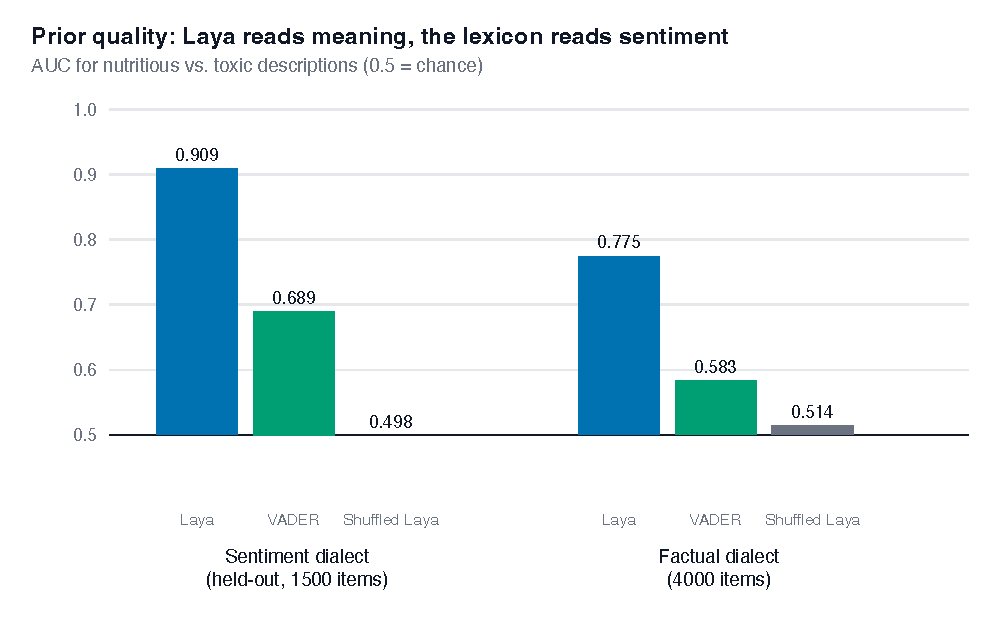
\includegraphics[width=0.75\textwidth]{figures/fig4_auc.pdf}
\caption{Quality of the prior: AUC for nutritious versus toxic descriptions (held-out field-notes dialect, 1,500 items; factual dialect, 4,000 items).}
\label{fig:auc}
\end{figure}

\subsection{The value of the prior depends on the delay of consequences}
\label{sec:res-delay}
\paragraph{An artefact of mismatched training.}
In pre-registration 04 the individuals were trained in worlds with a delay of 20 ticks and a deception rate of at most 0.25, and evaluated at delays 0 and 40 and at deception rates 0.25 and 0.40 (eight seeds). Without delay, individuals with the \laya{} prior were \emph{worse} than individuals with no prior in all eight seeds ($-0.085$ at deception 0.25, $-0.136$ at 0.40), while at delay 40 and deception 0.25 they were better ($+0.096$, 8/8). Read alone, this suggests that a prior harms when feedback is immediate.

\paragraph{Matched training removes the harm.}
In pre-registration 06 every training and evaluation world of a condition shares the same delay (48 runs, six seeds). Without delay the difference is $+0.015$ (interval $[-0.008,+0.052]$; four of six seeds positive); non-inferiority to a margin of $-0.04$ is supported, but the effect is not positive in every seed, so the correct reading is ``not harmful'', not ``helpful''. At delay 40 the difference is $+0.049$ ($[+0.025,+0.071]$, six of six seeds positive; supported). The harm in pre-registration 04 therefore came from evaluating individuals in worlds that differ from the ones they evolved in.

\paragraph{The value grows with the delay.}
In pre-registration 07 (eight new seeds, matched training, held-out dialect) the difference is $+0.038$ ($[+0.028,+0.048]$) at delay 40 and $+0.073$ ($[+0.069,+0.077]$) at delay 80; the per-seed values at delay 80 lie between 0.062 and 0.080. The growth with delay, (delay 80)$-$(delay 40), is $+0.035$ ($[+0.025,+0.046]$, 8/8; supported). At delay 80 individuals with the prior bit toxic food 386 times on average against 753 without it. Figure~\ref{fig:delay} shows the trend across the two pre-registrations. \textbf{This trend has to be read together with the behaviour of the no-prior genomes at delay 80.} On a shared sample of 12 held-out worlds, six of the eight no-prior genomes scored exactly as the blind rule that eats everything it reaches (fitness 0.253, 664 toxic bites, survival 0.357); the other two scored 0.264 and 0.266. At delay 40 all eight scored above the blind rule (0.288 to 0.305). In most seeds at delay 80, therefore, the experience-only learner did not learn to avoid anything, and part of the growth of the prior's value with the delay is the failure of this learner at long delays, not only the benefit of the prior. The blind rule and the oracle scored 0.253 and 0.563 on the same worlds, so individuals with the prior (0.352 to 0.377 across seeds) closed about a third of the gap between them. On the factual pool the corresponding differences are smaller ($+0.016$, interval containing zero, at delay 40; $+0.037$ at delay 80; descriptive). The pre-registration-04 hypothesis that the benefit at delay 40 reaches $+0.04$ was not supported: the mean was $+0.032$ in 8/8 seeds, and the interval $[+0.025,+0.042]$ contains the threshold (direction confirmed, magnitude unclear).

\begin{figure}[t]
\centering
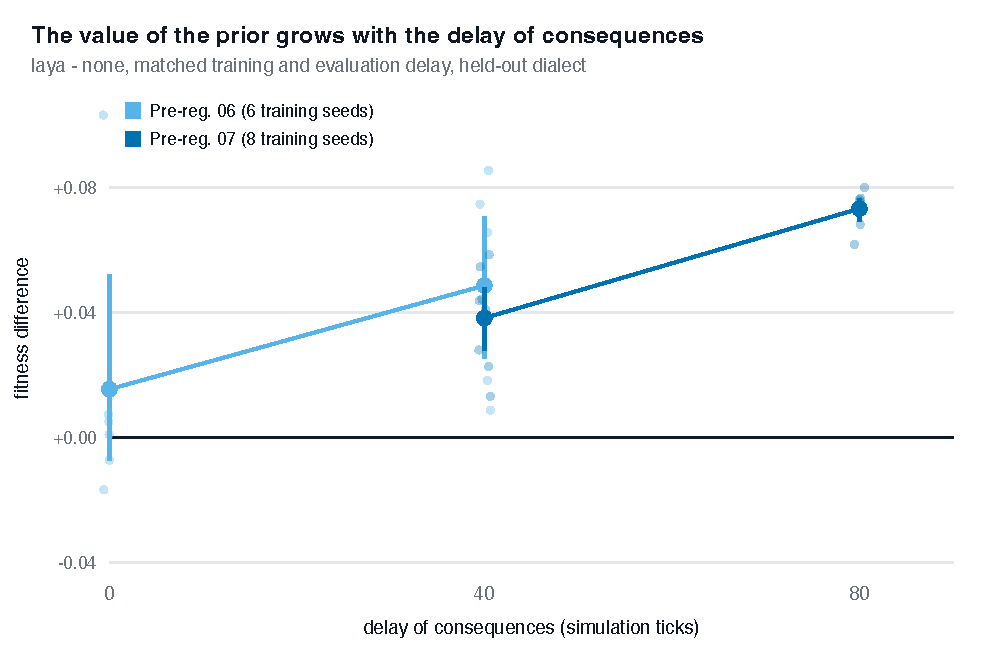
\includegraphics[width=0.75\textwidth]{figures/fig2_delay.pdf}
\caption{Fitness difference (\texttt{laya}$-$\texttt{none}) as a function of the consequence delay under matched training and evaluation, held-out dialect. Large dots are means with bootstrap intervals; small dots are training seeds.}
\label{fig:delay}
\end{figure}

\subsection{\laya{} versus a lexicon: only where meaning is needed}
\label{sec:res-lexicon}
In pre-registration 07, on the factual dialect at delay 40, individuals with the \laya{} prior beat individuals with the VADER prior by $+0.050$ ($[+0.038,+0.063]$, 8/8; supported). In the same worlds the VADER prior was worse than no prior ($-0.034$, seven of eight seeds negative; descriptive). On the held-out field-notes dialect, where the lexicon can read the text, the differences are smaller ($+0.025$ at delay 40, $+0.027$ at delay 80; descriptive, not tested).

Pre-registration 08 asked whether training on the factual dialect would widen the gap, and whether what is learned transfers. The gap did not widen: the difference \laya{}$-$VADER on the factual pool was $+0.029$ after sentiment-dialect training and $+0.028$ after factual-dialect training (change $-0.0015$, $[-0.008,+0.006]$; not supported). The advantage of the prior over no prior after factual training was $+0.032$ in 8/8 seeds, below the pre-registered threshold of 0.05 (not supported on magnitude). What \emph{did} differ was transfer to the held-out dialect: \laya{} individuals trained on the factual dialect scored 0.333 there, the same as those trained on the sentiment dialect (0.334), while VADER individuals fell from 0.307 to 0.271, so that \laya{}$-$VADER on the held-out pool grew from $+0.027$ to $+0.062$ ($[+0.058,+0.066]$, 8/8; the pre-registered non-inferiority test was supported). A plausible reading, which we have not tested, is that the reliability of a lexicon varies from dialect to dialect, so the trust that evolution assigns to it in one dialect does not carry over, whereas the reliability of the frozen model is stable and so is the trust learned for it.

In the ripening worlds (Section~\ref{sec:res-cues}), where the stage phrases carry sentiment that a lexicon can read, the two priors were indistinguishable ($+0.005$, $[-0.004,+0.013]$; not supported) or slightly in favour of the lexicon ($-0.014$ in the fair world, $[-0.027,-0.0005]$).

\subsection{Language cues are used, and wrong cues cost}
\label{sec:res-cues}
We evaluated the same individuals under three cue conditions (true, absent, mismatched; Section~\ref{sec:ecology}) with phrases that were never seen in training (Figure~\ref{fig:cues}).

\begin{figure}[t]
\centering
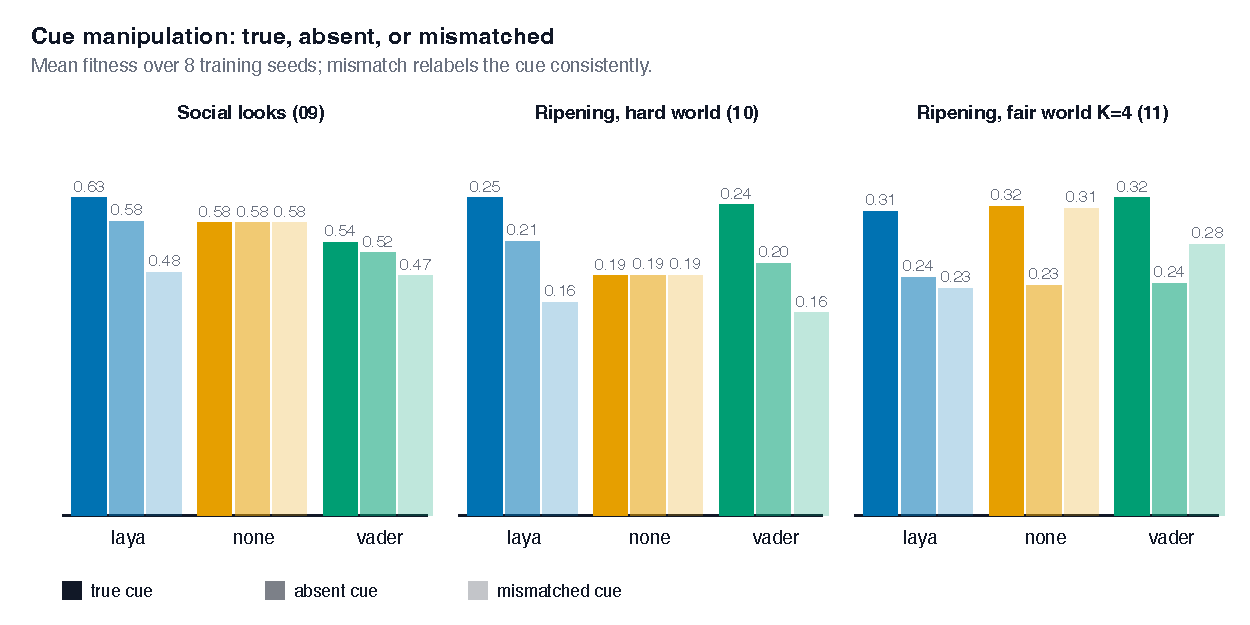
\includegraphics[width=\textwidth]{figures/fig3_cues.pdf}
\caption{Mean fitness under true, absent and mismatched cues, for individuals with each prior source (eight seeds). A mismatch relabels the cue consistently, so individuals that only learn from experience are unaffected; individuals that read the cue lose.}
\label{fig:cues}
\end{figure}

\paragraph{Social appearance (pre-registration 09).}
Individuals with the \laya{} prior scored 0.629 with true appearances, 0.582 with none and 0.481 with mismatched ones. The gain of true over absent appearances is $+0.047$ ($[+0.039,+0.055]$, 8/8; supported) and the cost of mismatched versus absent appearances $+0.101$ ($[+0.091,+0.111]$, 8/8; supported). Individuals with no prior were identical in all three conditions (0.579), as they cannot read the sentences. The gain was larger for \laya{} than for VADER individuals by $+0.025$ ($[+0.007,+0.044]$, $p=0.027$; supported under the pre-registered criteria, with the magnitude relative to the threshold unclear).

\paragraph{Ripening stages (pre-registration 10).}
In the hard ripening world ($K=16$) individuals with \laya{} scored 0.246, 0.212 and 0.165 under true, absent and mismatched stage phrases; VADER individuals 0.241, 0.195 and 0.157; no-prior individuals 0.186 under all three. The advantage of \laya{} over no prior was $+0.060$ ($[+0.044,+0.082]$, 8/8) and true versus mismatched cues $+0.081$ ($[+0.079,+0.083]$, 8/8); both were supported. But six of the eight no-prior individuals never ate (zero toxic bites), a degenerate strategy that evolution finds when experience alone cannot learn the world. The first result therefore mostly measures whether the individual can read the cue at all.

\subsection{When experience suffices, the prior adds nothing}
\label{sec:res-fair}
Pre-registration 11 repeated the ripening experiment in a world that experience-only individuals can learn ($K=4$): their fitness (0.315) lies between that of the blind rule (0.162) and that of the oracle (0.429), and one of eight never ate. Here individuals with \laya{} scored 0.310, 0.243 and 0.232 under true, absent and mismatched cues, those with no prior 0.315, 0.235 and 0.314, and those with VADER 0.324, 0.237 and 0.276. The difference \laya{}$-$none is $-0.005$ ($[-0.031,+0.032]$; not supported) and \laya{}$-$VADER is $-0.014$ ($[-0.027,-0.0005]$; not supported). The prior is still \emph{used}: true versus mismatched cues is $+0.079$ ($[+0.053,+0.097]$, 8/8; supported). But the mismatch costs only the individuals that read the phrase's meaning; the no-prior individuals, whose beliefs are keyed on the literal text, are unaffected (0.315 versus 0.314), and removing the cue entirely hurts everyone. In this one world, in which experience suffices, the net value of the prior is zero and it is not better than a lexicon; we have only this world and the harder one ($K=16$), so the result is not a dose--response relation between learnability and the value of a prior.

\subsection{Null and negative results}
\label{sec:res-null}
\begin{itemize}
\item \textbf{Hierarchical belief.} Letting an individual share evidence among similar descriptions, using the frozen encoder's embeddings, changed fitness by $+0.0005$ ($[-0.003,+0.004]$) for individuals with the \laya{} prior in the strongly deceptive worlds (pre-registration 06; not supported).
\item \textbf{An early large effect did not replicate.} With one training seed (pre-registration 02) \laya{} beat no prior by $+0.144$ ($[0.119,0.168]$) and a shuffled prior by $+0.155$. With three seeds (pre-registration 03) the differences against no prior were $+0.150$, $+0.011$ and $+0.039$ in seeds 1, 2 and 3; none of the three hypotheses was supported. The large effect was mainly due to the evolutionary outcome of the no-prior (and shuffled-prior) individuals in seed 1, which evolved poorly.
\item \textbf{The prior does not make outcomes more stable.} Across eight seeds the standard deviation of fitness was 0.0185 for individuals with the prior and 0.0084 for individuals without it (ratio 2.2), the opposite of the pre-registered hypothesis (pre-registration 04, not supported).
\end{itemize}

\section{Discussion}
\todo{Write after Results. Plan: PLAN.md, Discussion P1--P5 and Limitations (all items).}


\bibliographystyle{plainnat}
\bibliography{refs}

\appendix
\section{Tiered reading of all confirmatory comparisons}
\begin{table}[t]\centering\small\caption{Tiered reading of every confirmatory comparison. ``Direction confirmed means all seeds agree in sign (exact sign-flip $p=2^{-n}$); ``magnitude confirmed means the lower bound of the seed-level interval is at or above the pre-registered threshold; ``unclear means the interval contains it.}\label{tab:tiers}
\begin{tabular}{@{}lp{0.5\textwidth}rp{0.27\textwidth}@{}}\toprule
Pre-reg. & Comparison & Mean & Tiered reading \\\midrule
04 & Delay 40: laya $-$ none (mismatched training) & +0.032 & direction confirmed; magnitude unclear \\
04 & Prior value grows with delay (D40 $-$ D0) & +0.143 & direction confirmed; magnitude confirmed \\
06 & Delay 0: laya $-$ none (non-inferiority) & +0.015 & non-inferiority confirmed \\
06 & Delay 40: laya $-$ none (matched training) & +0.049 & direction confirmed; magnitude unclear \\
06 & Hierarchical belief, laya (deception 0.40) & +0.0005 & direction unclear; magnitude below threshold \\
07 & Factual dialect, delay 40: laya $-$ vader & +0.050 & direction confirmed; magnitude confirmed \\
07 & Held-out dialect, delay 80: laya $-$ none & +0.073 & direction confirmed; magnitude confirmed \\
07 & Prior value grows with delay (d80 $-$ d40) & +0.035 & direction confirmed; magnitude confirmed \\
08 & Gap widening: (laya $-$ vader) factual vs.\ sentiment training & -0.002 & direction unclear; magnitude below threshold \\
08 & Factual training: laya $-$ none (factual dialect) & +0.032 & direction confirmed; magnitude below threshold \\
08 & Transfer: factual-trained, held-out dialect, laya $-$ vader (non-inferiority) & +0.062 & non-inferiority confirmed \\
09 & Social looks: true $-$ absent (laya) & +0.047 & direction confirmed; magnitude confirmed \\
09 & Social looks: absent $-$ mismatched (laya) & +0.101 & direction confirmed; magnitude confirmed \\
09 & Social gain: laya $-$ vader & +0.025 & direction unclear; magnitude unclear \\
10 & Ripening: laya $-$ none (true cues) & +0.060 & direction confirmed; magnitude confirmed \\
10 & Ripening: true $-$ mismatched (laya) & +0.081 & direction confirmed; magnitude confirmed \\
10 & Ripening: laya $-$ vader & +0.005 & direction unclear; magnitude unclear \\
11 & Fair ripening ($K{=}4$): laya $-$ none & -0.005 & direction unclear; magnitude unclear \\
11 & Fair ripening: true $-$ mismatched (laya) & +0.079 & direction confirmed; magnitude confirmed \\
11 & Fair ripening: laya $-$ vader & -0.014 & direction unclear; magnitude below threshold \\
12 & Distilled head: distilled $-$ none (held-out, delay 80) & +0.045 & direction confirmed; magnitude confirmed \\
12 & Distilled head: non-inferiority to laya (held-out, delay 80) & -0.005 & non-inferiority confirmed \\
12 & Distilled head: laya $-$ distilled (factual, delay 80) & +0.045 & direction confirmed; magnitude confirmed \\
13 & Strong learner: none-lag $-$ none-plain (delay 80) & +0.165 & direction confirmed; magnitude confirmed \\
13 & Strong learner: laya-lag $-$ none-lag (delay 80) & +0.017 & direction unclear; magnitude unclear \\
13 & Strong learner: none-lag non-inferiority to laya-lag (delay 80) & -0.017 & non-inferiority unclear \\
13 & Strong learner: laya-lag $-$ laya-plain (delay 80) & +0.091 & direction confirmed; magnitude confirmed \\
14 & Other learners: none-safety $-$ none-plain (delay 80) & +0.0003 & direction unclear; magnitude below threshold \\
14 & Other learners: none-bayes $-$ none-plain (delay 80) & +0.009 & direction unclear; magnitude below threshold \\
14 & Other learners: shrinkage of the prior advantage under safety (delay 80) & +0.004 & direction unclear; magnitude below threshold \\
14 & Other learners: shrinkage of the prior advantage under bayes (delay 80) & +0.017 & direction confirmed; magnitude below threshold \\
15 & Variable delay (trained at fixed delay): none-lag $-$ none-plain, jitter & +0.112 & direction confirmed; magnitude confirmed \\
15 & Variable delay (trained at fixed delay): none-lag $-$ none-plain, per kind & -0.017 & direction unclear; magnitude below threshold \\
15 & Variable delay (trained at fixed delay): laya-lag $-$ laya-plain, jitter & +0.088 & direction confirmed; magnitude confirmed \\
15 & Variable delay (trained at fixed delay): laya-lag $-$ laya-plain, per kind & -0.097 & direction unclear; magnitude below threshold \\
15 & Variable delay (trained at fixed delay): laya-lag $-$ none-lag, pooled & +0.029 & direction unclear; magnitude unclear \\
16 & Variable delay (matched training): none-lag $-$ none-plain, jitter & +0.076 & direction confirmed; magnitude confirmed \\
16 & Variable delay (matched training): none-lag $-$ none-plain, per kind & -0.008 & direction unclear; magnitude below threshold \\
16 & Variable delay (matched training): laya-lag $-$ laya-plain, jitter & +0.041 & direction confirmed; magnitude unclear \\
16 & Variable delay (matched training): laya-lag $-$ laya-plain, per kind & +0.002 & direction unclear; magnitude below threshold \\
16 & Variable delay (matched training): laya-lag $-$ none-lag, pooled & +0.002 & direction unclear; magnitude below threshold \\
17 & Retention: regime $-$ plain savings (A/B/A, no cue) & +0.215 & direction confirmed; magnitude confirmed \\
17 & Retention: cue $-$ plain savings (A/B/A, true cue) & +0.345 & direction confirmed; magnitude confirmed \\
17 & Retention: cue $-$ regime savings (A/B/A, true cue) & +0.126 & direction confirmed; magnitude confirmed \\
17 & New rule: regime non-inferior to plain (A/B/C, no cue) & +0.024 & non-inferiority confirmed \\
17 & Random cue: plain $-$ cue fitness (A/B/A) & -0.159 & direction unclear; magnitude below threshold \\
17 & Retention: regime $-$ plain fitness (A/B/A, no cue) & +0.084 & direction confirmed; magnitude confirmed \\
03 & laya $-$ shuffled (3 seeds) & +0.066 & direction confirmed \\
03 & laya $-$ none (3 seeds) & +0.067 & direction confirmed \\
03 & laya $-$ vader (3 seeds) & +0.012 & direction unclear \\
\bottomrule\end{tabular}\end{table}

\section{Pre-registration 03 and all rows}
\begin{table}[t]\centering\small\caption{All confirmatory comparisons including pre-registration 03, with the tiered reading of each result in the last column of the supplementary table.}\label{tab:all}
\resizebox{\textwidth}{!}{\begin{tabular}{@{}llrrrrll@{}}\toprule
Pre-reg. & Comparison & $n$ & Mean & 95\% interval & $p$ & Threshold & Formal outcome \\\midrule
04 & Delay 40: laya $-$ none (mismatched training) & 8 & +0.032 & [+0.025, +0.042] & 0.0039 & +0.04 & not supported (magnitude) \\
04 & Prior value grows with delay (D40 $-$ D0) & 8 & +0.143 & [+0.120, +0.168] & 0.0039 & +0.03 & not claimed (tied $p$) \\
06 & Delay 0: laya $-$ none (non-inferiority) & 6 & +0.015 & [-0.008, +0.052] & 0.0156 & -0.04 & supported \\
06 & Delay 40: laya $-$ none (matched training) & 6 & +0.049 & [+0.025, +0.071] & 0.0156 & +0.04 & supported \\
06 & Hierarchical belief, laya (deception 0.40) & 6 & +0.0005 & [-0.003, +0.004] & 0.4375 & +0.03 & not supported \\
07 & Factual dialect, delay 40: laya $-$ vader & 8 & +0.050 & [+0.038, +0.063] & 0.0039 & +0.03 & supported \\
07 & Held-out dialect, delay 80: laya $-$ none & 8 & +0.073 & [+0.069, +0.077] & 0.0039 & +0.04 & supported \\
07 & Prior value grows with delay (d80 $-$ d40) & 8 & +0.035 & [+0.025, +0.046] & 0.0039 & +0.02 & supported \\
08 & Gap widening: (laya $-$ vader) factual vs.\ sentiment training & 8 & -0.002 & [-0.008, +0.006] & 0.6328 & +0.02 & not supported \\
08 & Factual training: laya $-$ none (factual dialect) & 8 & +0.032 & [+0.026, +0.038] & 0.0039 & +0.05 & not supported (magnitude) \\
08 & Transfer: factual-trained, held-out dialect, laya $-$ vader (non-inferiority) & 8 & +0.062 & [+0.058, +0.066] & 0.0039 & -0.02 & supported \\
09 & Social looks: true $-$ absent (laya) & 8 & +0.047 & [+0.039, +0.055] & 0.0039 & +0.02 & supported \\
09 & Social looks: absent $-$ mismatched (laya) & 8 & +0.101 & [+0.091, +0.111] & 0.0039 & +0.05 & supported \\
09 & Social gain: laya $-$ vader & 8 & +0.025 & [+0.007, +0.044] & 0.0273 & +0.01 & supported \\
10 & Ripening: laya $-$ none (true cues) & 8 & +0.060 & [+0.044, +0.082] & 0.0039 & +0.03 & supported \\
10 & Ripening: true $-$ mismatched (laya) & 8 & +0.081 & [+0.079, +0.083] & 0.0039 & +0.05 & supported \\
10 & Ripening: laya $-$ vader & 8 & +0.005 & [-0.003, +0.013] & 0.1328 & +0.01 & not supported \\
11 & Fair ripening ($K{=}4$): laya $-$ none & 8 & -0.005 & [-0.031, +0.032] & 0.5938 & +0.03 & not supported \\
11 & Fair ripening: true $-$ mismatched (laya) & 8 & +0.079 & [+0.053, +0.097] & 0.0039 & +0.05 & supported \\
11 & Fair ripening: laya $-$ vader & 8 & -0.014 & [-0.027, -0.0005] & 0.9492 & +0.01 & not supported \\
12 & Distilled head: distilled $-$ none (held-out, delay 80) & 8 & +0.045 & [+0.036, +0.054] & 0.0039 & +0.03 & supported \\
12 & Distilled head: non-inferiority to laya (held-out, delay 80) & 8 & -0.005 & [-0.011, +0.003] & 0.0039 & -0.03 & supported \\
12 & Distilled head: laya $-$ distilled (factual, delay 80) & 8 & +0.045 & [+0.037, +0.054] & 0.0039 & +0.01 & supported \\
13 & Strong learner: none-lag $-$ none-plain (delay 80) & 8 & +0.165 & [+0.142, +0.182] & 0.0039 & +0.10 & supported \\
13 & Strong learner: laya-lag $-$ none-lag (delay 80) & 8 & +0.017 & [-0.004, +0.048] & 0.1914 & +0.02 & not supported \\
13 & Strong learner: none-lag non-inferiority to laya-lag (delay 80) & 8 & -0.017 & [-0.048, +0.004] & 0.4375 & -0.02 & not supported \\
13 & Strong learner: laya-lag $-$ laya-plain (delay 80) & 8 & +0.091 & [+0.075, +0.106] & 0.0039 & +0.03 & supported \\
14 & Other learners: none-safety $-$ none-plain (delay 80) & 8 & +0.0003 & [-0.008, +0.008] & 0.5000 & +0.05 & not supported \\
14 & Other learners: none-bayes $-$ none-plain (delay 80) & 8 & +0.009 & [+0.002, +0.016] & 0.0234 & +0.05 & not supported \\
14 & Other learners: shrinkage of the prior advantage under safety (delay 80) & 8 & +0.004 & [-0.003, +0.011] & 0.1445 & +0.03 & not supported \\
14 & Other learners: shrinkage of the prior advantage under bayes (delay 80) & 8 & +0.017 & [+0.008, +0.026] & 0.0039 & +0.03 & 不成立（Holm 拒绝，效应量未达） \\
15 & Variable delay (trained at fixed delay): none-lag $-$ none-plain, jitter & 8 & +0.112 & [+0.085, +0.143] & 0.0039 & +0.03 & 成立（训练缺陷） \\
15 & Variable delay (trained at fixed delay): none-lag $-$ none-plain, per kind & 8 & -0.017 & [-0.030, -0.006] & 0.9883 & +0.03 & 不成立（训练缺陷） \\
15 & Variable delay (trained at fixed delay): laya-lag $-$ laya-plain, jitter & 8 & +0.088 & [+0.062, +0.112] & 0.0039 & +0.03 & 成立（训练缺陷） \\
15 & Variable delay (trained at fixed delay): laya-lag $-$ laya-plain, per kind & 8 & -0.097 & [-0.113, -0.080] & 1.0000 & +0.03 & 不成立（训练缺陷） \\
15 & Variable delay (trained at fixed delay): laya-lag $-$ none-lag, pooled & 8 & +0.029 & [+0.014, +0.044] & 0.0078 & +0.02 & 成立（训练缺陷） \\
03 & laya $-$ shuffled (3 seeds) & 3 & +0.066 & [+0.012, +0.147] & 0.1250 &  & not supported (intersection) \\
03 & laya $-$ none (3 seeds) & 3 & +0.067 & [+0.011, +0.150] & 0.1250 &  & not supported (intersection) \\
03 & laya $-$ vader (3 seeds) & 3 & +0.012 & [-0.010, +0.031] & 0.2500 &  & not supported (intersection) \\
\bottomrule\end{tabular}}\end{table}


\end{document}
